% ============================================================
\chapter{Introduction \`a la Recherche Op\'erationnelle}
\label{ch:introduction}
% ============================================================

Pendant la Seconde Guerre mondiale, la Royal Air Force britannique fait face
\`a un probl\`eme logistique d\'esesp\'erant~: comment d\'eployer ses radars
c\^otiers pour d\'etecter les bombardiers ennemis avec un nombre limit\'e de
stations~? Un groupe de scientifiques --- physiciens, math\'ematiciens,
biologistes --- est r\'euni pour analyser le probl\`eme
\emph{op\'erationnellement}, c'est-\`a-dire avec des donn\'ees, des mod\`eles
et des m\'ethodes quantitatives. Ils appellent leur discipline
\og operational research\fg, et les r\'esultats sont spectaculaires~: les
pertes diminuent, l'efficacit\'e monte. Apr\`es la guerre, ces m\'ethodes
migrent vers l'industrie, les transports, la sant\'e et la finance,
devenant ce que nous appelons aujourd'hui la \emph{recherche
op\'erationnelle}.

Ce chapitre trace les contours de cette discipline~: ses origines, sa
d\'emarche, et les grandes classes de probl\`emes qu'elle cherche \`a
r\'esoudre.

% ------------------------------------------------------------
\section{Qu'est-ce que la recherche op\'erationnelle~?}
% ------------------------------------------------------------

Commen\c{c}ons par d\'efinir pr\'ecis\'ement l'objet de notre \'etude.

\begin{definition}[Recherche op\'erationnelle]
La \textbf{recherche op\'erationnelle} (RO) est l'application de m\'ethodes
scientifiques --- math\'ematiques, statistiques et informatiques --- \`a la prise
de d\'ecision dans les syst\`emes complexes.  Son objectif est de d\'eterminer la
meilleure allocation de ressources limit\'ees pour atteindre un but donn\'e.
\end{definition}

La RO se distingue des autres branches des math\'ematiques appliqu\'ees par son
ancrage dans la \emph{mod\'elisation} de probl\`emes r\'eels et par le souci
constant de fournir des solutions \emph{impl\'ementables}.

\begin{remarque}
Le terme \og recherche op\'erationnelle \fg vient de l'anglais
\textit{Operations Research}, o\`u \textit{operations} d\'esigne les op\'erations
militaires au cours desquelles la discipline est n\'ee.  En fran\c{c}ais, on
utilise parfois l'abr\'eviation \textbf{RO}.
\end{remarque}

\section{Bref historique}

\subsection{Les origines militaires (1937--1945)}

Les pr\'emisses de la RO remontent aux travaux de \textbf{Leonid Kantorovich}
(1937) sur l'optimisation de la production dans l'industrie sovi\'etique.
Cependant, la discipline prend v\'eritablement son essor pendant la Seconde
Guerre mondiale~:

\begin{itemize}
  \item En \textbf{1940}, le physicien Patrick Blackett dirige le
        \textit{Blackett's Circus}, un groupe interdisciplinaire charg\'e
        d'optimiser le d\'eploiement des radars et la taille des convois
        maritimes.
  \item Aux \'Etats-Unis, des \'equipes similaires travaillent sur la strat\'egie
        de bombardement et la logistique du Pacifique.
\end{itemize}

\subsection{L'\`ere fondatrice (1947--1960)}

\begin{itemize}
  \item \textbf{1947}~: George \textbf{Dantzig} invente la \textbf{m\'ethode du
        simplexe} pour r\'esoudre les programmes lin\'eaires.
  \item \textbf{1951}~: Harold \textbf{Kuhn} et Albert \textbf{Tucker}
        formalisent les conditions d'optimalit\'e en programmation non lin\'eaire
        (conditions KKT).
  \item \textbf{1956}~: Lester \textbf{Ford} et Delbert \textbf{Fulkerson}
        publient l'algorithme du flot maximal.
  \item \textbf{1958}~: Ralph \textbf{Gomory} introduit la m\'ethode des
        coupes enti\`eres.
  \item \textbf{1960}~: Ailsa \textbf{Land} et Alison \textbf{Doig}
        formalisent le \textbf{branch-and-bound}.
\end{itemize}

\subsection{D\'eveloppements modernes}

\begin{itemize}
  \item \textbf{1979}~: Leonid \textbf{Khachiyan} d\'emontre que la
        programmation lin\'eaire est r\'esoluble en temps polynomial (m\'ethode de
        l'ellipso\"ide).
  \item \textbf{1984}~: Narendra \textbf{Karmarkar} publie la m\'ethode des
        points int\'erieurs, comp\'etitive avec le simplexe en pratique.
  \item \textbf{Ann\'ees 2000--2020}~: Les solveurs modernes (CPLEX, Gurobi,
        CBC) r\'esolvent des probl\`emes \`a des millions de variables.
\end{itemize}

\section{Domaines d'application}

La RO intervient dans de tr\`es nombreux secteurs~:

\begin{center}
\renewcommand{\arraystretch}{1.2}
\begin{tabular}{ll}
  \toprule
  \textbf{Secteur} & \textbf{Exemples de probl\`emes} \\
  \midrule
  Logistique & Planification de tourn\'ees, gestion de stocks \\
  Production & Ordonnancement, dimensionnement de lots \\
  Finance & Optimisation de portefeuille, gestion du risque \\
  Transport & Conception de r\'eseaux, horaires de bus/trains \\
  T\'el\'ecommunications & Routage, affectation de fr\'equences \\
  Sant\'e & Planification des blocs op\'eratoires, gestion de lits \\
  \'Energie & Unit commitment, gestion de r\'eseaux \'electriques \\
  A\'eronautique & Revenue management, affectation de portes \\
  \bottomrule
\end{tabular}
\end{center}

\section{M\'ethodologie de la RO}

La d\'emarche g\'en\'erale de la RO suit un cycle en six \'etapes~:

\begin{enumerate}
  \item \textbf{D\'efinition du probl\`eme}~: identifier l'objectif, les
        d\'ecideurs, les contraintes op\'erationnelles.
  \item \textbf{Collecte des donn\'ees}~: param\`etres du mod\`ele, co\^uts,
        capacit\'es, demandes.
  \item \textbf{Formulation du mod\`ele}~: traduire le probl\`eme en termes
        math\'ematiques (variables, objectif, contraintes).
  \item \textbf{R\'esolution}~: appliquer un algorithme ou un solveur.
  \item \textbf{Validation}~: v\'erifier la coh\'erence du mod\`ele et la
        pertinence de la solution.
  \item \textbf{Impl\'ementation}~: mettre en \oe uvre la solution et suivre
        ses performances.
\end{enumerate}

\begin{intuition}[title=\textbf{Mod\'eliser, c'est simplifier}]
Un mod\`ele n'est jamais une repr\'esentation exacte de la r\'ealit\'e.
L'art de la mod\'elisation consiste \`a trouver le bon \'equilibre entre
\emph{pr\'ecision} (mod\`ele fid\`ele) et \emph{tractabilit\'e} (mod\`ele
r\'esoluble).
\end{intuition}

\section{Classification des mod\`eles d'optimisation}

\begin{definition}[Probl\`eme d'optimisation]
Un \textbf{probl\`eme d'optimisation} se formule de mani\`ere g\'en\'erique
comme~:
\[
  \min_{\mathbf{x} \in \mathcal{X}} f(\mathbf{x})
  \quad \text{sous les contraintes} \quad
  g_i(\mathbf{x}) \le 0, \; i = 1, \ldots, m,
  \qquad
  h_j(\mathbf{x}) = 0, \; j = 1, \ldots, p,
\]
o\`u $f$ est la \textbf{fonction objectif}, $\mathcal{X}$ l'ensemble de
d\'efinition, les $g_i$ les \textbf{contraintes d'in\'egalit\'e} et les $h_j$
les \textbf{contraintes d'\'egalit\'e}.
\end{definition}

On distingue les mod\`eles selon plusieurs crit\`eres~:

\subsection{Selon la nature de l'objectif et des contraintes}

\begin{itemize}
  \item \textbf{Programmation lin\'eaire (PL)}~: $f$, $g_i$, $h_j$ sont des
        fonctions lin\'eaires de $\mathbf{x}$.
  \item \textbf{Programmation non lin\'eaire (PNL)}~: au moins l'une des
        fonctions est non lin\'eaire.
  \item \textbf{Programmation quadratique}~: objectif quadratique,
        contraintes lin\'eaires.
\end{itemize}

\subsection{Selon la nature des variables}

\begin{itemize}
  \item \textbf{Variables continues}~: $\mathbf{x} \in \R^n$.
  \item \textbf{Variables enti\`eres}~: $\mathbf{x} \in \Z^n$
        (programmation en nombres entiers, PLNE).
  \item \textbf{Variables mixtes}~: certaines continues, d'autres enti\`eres
        (programmation mixte, MIP).
  \item \textbf{Variables binaires}~: $x_i \in \{0, 1\}$
        (programmation 0--1).
\end{itemize}

\subsection{Selon l'information disponible}

\begin{itemize}
  \item \textbf{D\'eterministe}~: tous les param\`etres sont connus avec
        certitude.
  \item \textbf{Stochastique}~: certains param\`etres sont des variables
        al\'eatoires.
  \item \textbf{Robuste}~: on cherche une solution performante pour tous
        les sc\'enarios possibles.
\end{itemize}

\section{Premiers exemples de mod\'elisation}

\begin{exemple}[Probl\`eme de production]
Une usine fabrique deux produits $P_1$ et $P_2$.  Chaque unit\'e de $P_1$
rapporte 5\,EUR et n\'ecessite 2~heures de machine~A et 1~heure de
machine~B.  Chaque unit\'e de $P_2$ rapporte 4\,EUR et n\'ecessite 1~heure
de machine~A et 3~heures de machine~B.  La machine~A est disponible
10~heures par jour, la machine~B 12~heures.

\textbf{Variables de d\'ecision}~:
$x_1$ = nombre d'unit\'es de $P_1$, $x_2$ = nombre d'unit\'es de $P_2$.

\textbf{Mod\`ele}~:
\[
\begin{aligned}
  \max \quad & z = 5x_1 + 4x_2 \\
  \text{s.c.} \quad
    & 2x_1 + x_2 \le 10 & \text{(machine A)} \\
    & x_1 + 3x_2 \le 12  & \text{(machine B)} \\
    & x_1, x_2 \ge 0
\end{aligned}
\]
\end{exemple}

\begin{exemple}[Probl\`eme de m\'elange]
Un \'eleveur souhaite pr\'eparer un m\'elange alimentaire pour ses animaux au
moindre co\^ut.  Deux ingr\'edients sont disponibles~:

\begin{center}
\begin{tabular}{lccc}
  \toprule
  & Prot\'eines (\%/kg) & Lipides (\%/kg) & Co\^ut (EUR/kg) \\
  \midrule
  Ingr\'edient 1 & 20 & 5 & 3 \\
  Ingr\'edient 2 & 10 & 8 & 2 \\
  \midrule
  Besoin minimal & 15 & 6 & --- \\
  \bottomrule
\end{tabular}
\end{center}

Soit $x_1, x_2$ les quantit\'es (en kg) des deux ingr\'edients.  Le m\'elange
doit peser 1~kg~: $x_1 + x_2 = 1$.

\[
\begin{aligned}
  \min \quad & z = 3x_1 + 2x_2 \\
  \text{s.c.} \quad
    & 20x_1 + 10x_2 \ge 15 & \text{(prot\'eines)} \\
    & 5x_1 + 8x_2 \ge 6   & \text{(lipides)} \\
    & x_1 + x_2 = 1 \\
    & x_1, x_2 \ge 0
\end{aligned}
\]
\end{exemple}

\section{R\'esolution graphique (aper\c{c}u)}

Pour les probl\`emes \`a deux variables, on peut repr\'esenter l'ensemble
r\'ealisable dans le plan et trouver l'optimum graphiquement.

\begin{center}
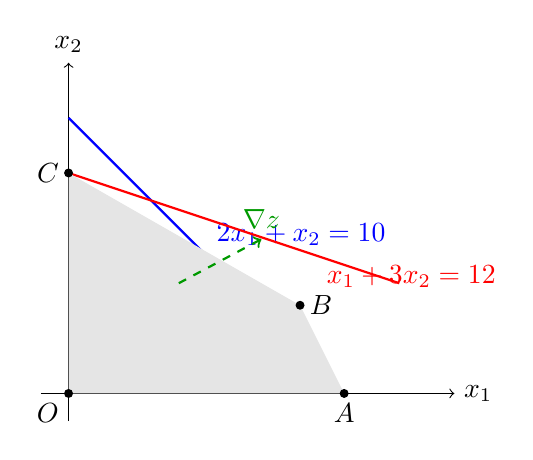
\begin{tikzpicture}[scale=0.7]
  % Axes
  \draw[->] (-0.5,0) -- (7,0) node[right] {$x_1$};
  \draw[->] (0,-0.5) -- (0,6) node[above] {$x_2$};
  % Contrainte 1 : 2x1 + x2 <= 10
  \draw[thick, blue] (0,10*0.5) -- (5,0)
    node[midway, above right] {$2x_1+x_2=10$};
  % Contrainte 2 : x1 + 3x2 <= 12
  \draw[thick, red] (0,4) -- (6,2)
    node[near end, below right] {$x_1+3x_2=12$};
  % Zone réalisable (remplissage)
  \fill[gray!20] (0,0) -- (5,0) -- (4.2,1.6) -- (0,4) -- cycle;
  % Sommets
  \filldraw (0,0) circle (2pt) node[below left] {$O$};
  \filldraw (5,0) circle (2pt) node[below] {$A$};
  \filldraw (4.2,1.6) circle (2pt) node[right] {$B$};
  \filldraw (0,4) circle (2pt) node[left] {$C$};
  % Direction gradient
  \draw[->, thick, dashed, green!60!black] (2,2) -- (3.5,2.8)
    node[above] {$\nabla z$};
\end{tikzpicture}
\end{center}

Le sommet $B = (4.2, 1.6)$ maximise $z = 5(4.2) + 4(1.6) = 27.4$.
On retrouvera ce r\'esultat formellement au chapitre~3 par la m\'ethode du
simplexe.

\section{Introduction aux solveurs}

\begin{codeblock}[title=\textbf{R\'esolution avec SciPy}]
\begin{minted}{python}
from scipy.optimize import linprog

# min c^T x  =>  on maximise en changeant le signe
c = [-5, -4]  # max 5x1 + 4x2

# Contraintes : A_ub @ x <= b_ub
A_ub = [[2, 1],   # 2x1 + x2 <= 10
        [1, 3]]   # x1 + 3x2 <= 12
b_ub = [10, 12]

# Bornes : x1, x2 >= 0
x_bounds = (0, None)
bounds = [x_bounds, x_bounds]

result = linprog(c, A_ub=A_ub, b_ub=b_ub, bounds=bounds,
                 method='highs')
print(f"x* = {result.x}")
print(f"z* = {-result.fun:.2f}")
\end{minted}
\end{codeblock}

\begin{codeoutput}
x* = [4.2 1.6]
z* = 27.40
\end{codeoutput}

\begin{codeblock}[title=\textbf{R\'esolution avec PuLP}]
\begin{minted}{python}
import pulp

prob = pulp.LpProblem("Production", pulp.LpMaximize)

x1 = pulp.LpVariable("x1", lowBound=0)
x2 = pulp.LpVariable("x2", lowBound=0)

# Objectif
prob += 5*x1 + 4*x2, "Profit"

# Contraintes
prob += 2*x1 + x2 <= 10, "Machine_A"
prob += x1 + 3*x2 <= 12, "Machine_B"

prob.solve(pulp.PULP_CBC_CMD(msg=0))

print(f"Statut : {pulp.LpStatus[prob.status]}")
print(f"x1 = {x1.varValue}, x2 = {x2.varValue}")
print(f"Profit = {pulp.value(prob.objective):.2f}")
\end{minted}
\end{codeblock}

\begin{codeoutput}
Statut : Optimal
x1 = 4.2, x2 = 1.6
Profit = 27.40
\end{codeoutput}

\section{Complexit\'e algorithmique~: rappels}

\begin{definition}[Notation $\mathcal{O}$]
On dit qu'un algorithme a une complexit\'e en $\mathcal{O}(g(n))$ s'il existe
des constantes $C > 0$ et $n_0$ telles que le nombre d'op\'erations \'el\'ementaires
est major\'e par $C \cdot g(n)$ pour tout $n \ge n_0$.
\end{definition}

\begin{center}
\renewcommand{\arraystretch}{1.2}
\begin{tabular}{lll}
  \toprule
  \textbf{Classe} & \textbf{Complexit\'e} & \textbf{Exemple} \\
  \midrule
  $\mathcal{P}$ & Polynomial & Simplexe (en pratique), Dijkstra \\
  $\mathcal{NP}$ & V\'erifiable en temps polynomial & Probl\`eme du sac \`a dos \\
  $\mathcal{NP}$-complet & Aussi dur que tout probl\`eme $\mathcal{NP}$ & TSP (d\'ecision) \\
  $\mathcal{NP}$-difficile & Au moins aussi dur que $\mathcal{NP}$-complet & TSP (optimisation) \\
  \bottomrule
\end{tabular}
\end{center}

\begin{attention}[title=\textbf{Complexit\'e du simplexe}]
Bien que le simplexe soit en temps exponentiel dans le pire cas (exemples de
Klee-Minty), il est extr\^emement efficace en pratique.  Les m\'ethodes de
points int\'erieurs offrent une complexit\'e polynomiale garantie~:
$\mathcal{O}(n^{3.5} L)$ o\`u $L$ est la taille de l'entr\'ee.
\end{attention}

\section{Vocabulaire fondamental}

\begin{definition}[Solution r\'ealisable]
Une solution $\mathbf{x}$ est dite \textbf{r\'ealisable} (ou \textbf{admissible})
si elle satisfait toutes les contraintes du probl\`eme.
L'ensemble des solutions r\'ealisables est not\'e $\mathcal{F}$ (\textit{feasible set}).
\end{definition}

\begin{definition}[Solution optimale]
Une solution r\'ealisable $\mathbf{x}^*$ est \textbf{optimale} si
$f(\mathbf{x}^*) \le f(\mathbf{x})$ pour tout $\mathbf{x} \in \mathcal{F}$
(dans le cas d'une minimisation).
\end{definition}

\begin{definition}[Probl\`eme non born\'e]
Un probl\`eme est dit \textbf{non born\'e} si la fonction objectif peut prendre
des valeurs arbitrairement petites (minimisation) ou grandes (maximisation)
sur $\mathcal{F}$.
\end{definition}

\begin{definition}[Probl\`eme non r\'ealisable]
Un probl\`eme est dit \textbf{non r\'ealisable} (\textit{infeasible}) si
$\mathcal{F} = \emptyset$, c'est-\`a-dire si aucune solution ne satisfait
simultan\'ement toutes les contraintes.
\end{definition}

\section{Exercices}

\begin{exercice}[$\star$ -- Mod\'elisation]
Une entreprise fabrique trois produits $A$, $B$ et $C$ avec les donn\'ees
suivantes~:

\begin{center}
\begin{tabular}{lcccc}
  \toprule
  & Machine~1 (h) & Machine~2 (h) & Machine~3 (h) & Profit (EUR) \\
  \midrule
  $A$ & 1 & 2 & 1 & 10 \\
  $B$ & 2 & 1 & 3 & 15 \\
  $C$ & 1 & 1 & 2 & 12 \\
  \midrule
  Disponibilit\'e & 40 & 50 & 60 & \\
  \bottomrule
\end{tabular}
\end{center}

Formuler le programme lin\'eaire qui maximise le profit total.
\end{exercice}

\begin{exercice}[$\star$ -- R\'esolution graphique]
R\'esoudre graphiquement~:
\[
\begin{aligned}
  \max \quad & z = 3x_1 + 2x_2 \\
  \text{s.c.} \quad
    & x_1 + x_2 \le 4 \\
    & x_1 + 3x_2 \le 6 \\
    & x_1, x_2 \ge 0
\end{aligned}
\]
\end{exercice}

\begin{exercice}[$\star\star$ -- Probl\`eme de r\'egime alimentaire]
Un di\'et\'eticien doit composer un repas \`a co\^ut minimal contenant au moins
2000~kcal, 55~g de prot\'eines et 800~mg de calcium.  Quatre aliments sont
disponibles avec les donn\'ees suivantes~:

\begin{center}
\begin{tabular}{lcccc}
  \toprule
  & kcal/100g & Prot\'eines (g/100g) & Calcium (mg/100g) & Co\^ut (EUR/100g) \\
  \midrule
  Pain & 265 & 9 & 15 & 0.30 \\
  Lait & 65 & 3.5 & 120 & 0.15 \\
  Fromage & 350 & 25 & 700 & 1.20 \\
  Pomme & 52 & 0.3 & 6 & 0.40 \\
  \bottomrule
\end{tabular}
\end{center}

Formuler le PL correspondant.
\end{exercice}

\begin{exercice}[$\star\star$ -- Code Python]
Impl\'ementer et r\'esoudre le probl\`eme de l'exercice~1 avec PuLP.
V\'erifier le r\'esultat avec \texttt{scipy.optimize.linprog}.
\end{exercice}

\begin{exercice}[$\star\star\star$ -- Mod\'elisation avec variables binaires]
Un investisseur dispose de 100\,000\,EUR et doit choisir parmi 5~projets
d'investissement.  Chaque projet $i$ n\'ecessite un investissement de $c_i$ et
rapporte $r_i$.  L'investisseur ne peut investir que dans un projet en entier
(pas de fraction).  De plus, s'il investit dans le projet~3, il doit aussi
investir dans le projet~1.  Formuler ce probl\`eme comme un programme lin\'eaire
en nombres entiers (PLNE).
\end{exercice}
